\documentclass[12pt]{article}
\usepackage{geometry}                % See geometry.pdf to learn the layout options. There are lots.
\geometry{letterpaper}                   % ... or a4paper or a5paper or ... 
%\geometry{landscape}                % Activate for for rotated page geometry
\usepackage[parfill]{parskip}    % Activate to begin paragraphs with an empty line rather than an indent
\usepackage{daves,fancyhdr,natbib,graphicx,dcolumn,amsmath,lastpage,url}
\usepackage{amsmath,amssymb,epstopdf,longtable}
\DeclareGraphicsRule{.tif}{png}{.png}{`convert #1 `dirname #1`/`basename #1 .tif`.png}
\pagestyle{fancy}
\lhead{CE 3372 -- Water Systems Design}
\rhead{SPRING 2025}
\lfoot{EXERCISE 13}
\cfoot{}
\rfoot{Page \thepage\ of \pageref{LastPage}}
\renewcommand\headrulewidth{0pt}


\begin{document}
\begin{center}
{\textbf{{ CE 3372 -- Water Systems Design} \\ {Exercise Set 13}}}
\end{center}
\section*{\small{Purpose:}}
Demonstrate conduit sizing using Rational equation method for eventual application of SWMM for analysis of a storm drainage system.
\section*{\small{Objectives:}}
\begin{itemize}
\item Determine drainage areas to each inlet
\item Determine inlet times and pipe travel times, to size conduits for a storm drain system.
\item Prepare data for hydraulic model testing in SWMM
\end{itemize}

\section*{\small{Problem Statement and Background}}
Figure \ref{fig:aerial} is an older (circa 1993) aerial image of a portion of Houston, Texas.   
The red polygon is the drainage boundary for a storm sewer system that drains North from the part of the area near Westheimer Road to a tributary of Buffalo Bayou and East from the area.
The drainage ditch is shown as the ``blue''   fuzzy line on the figure.  
Drainage in the ditch is from West to East.
The two main streets in the study area are highlighted in magenta.  

\begin{figure}[h!] %  figure placement: here, top, bottom, or page
   \centering
   \includegraphics[height=7in]{Image118.jpg} 
   \caption{Tanglewilde Drive Study Area}
   \label{fig:aerial}
\end{figure}
\clearpage

Figure \ref{fig:survey} is a map showing storm drainage alignments and inlets location.  
\begin{figure}[h!] %  figure placement: here, top, bottom, or page
   \centering
   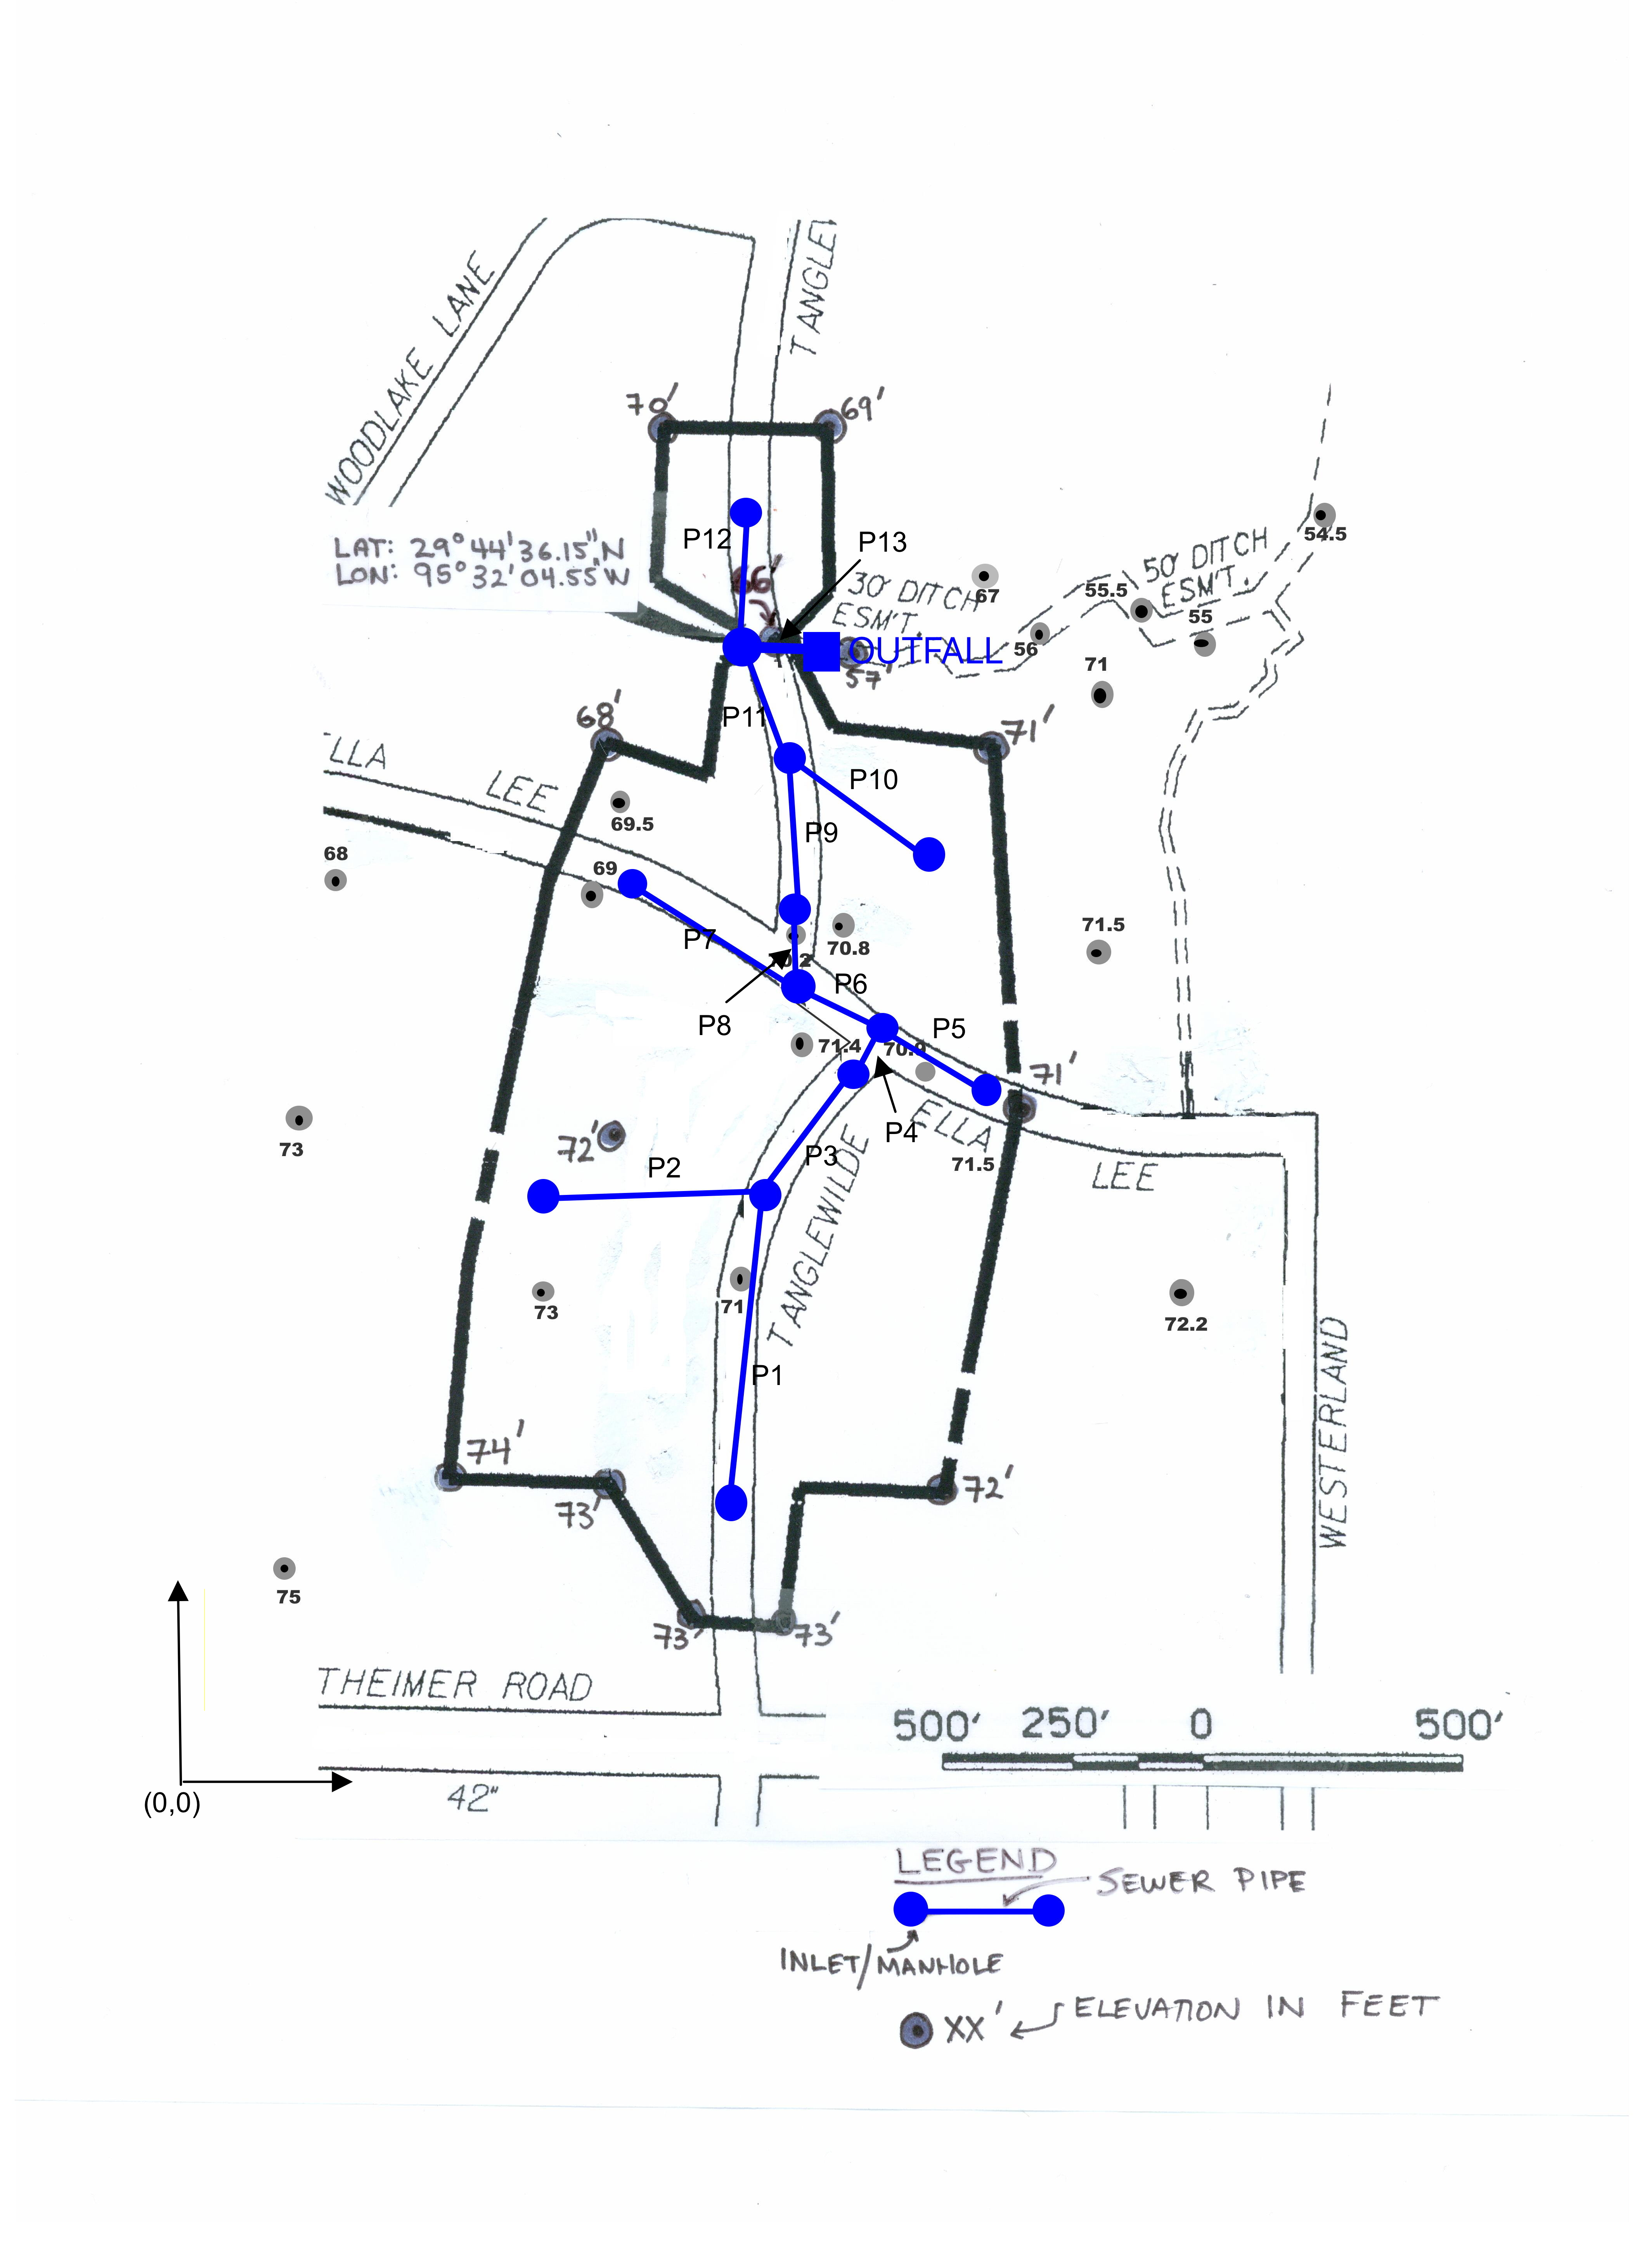
\includegraphics[height=7in]{Image119B.jpg} 
   \caption{Tanglewilde Drive Storm Drain Inlet and Pipe Alignments}
   \label{fig:survey}
\end{figure}

The figure shows land surface elevations in feet at the indicated locations.  
A linear scale is shown in the legend.  
Use the map(s) and:

\begin{enumerate}
\item Constructed a contour map of the same area. Use the contour map to inform your selection of the drainage areas to each inlet node. Indicate which nodes you do not assign drainage (junction nodes for connecting pipes).
\item Use the rational design method to size the conduits for a 5-year storm, for Harris County, Texas.
\item Specify the invert (flow line) elevations of the nodes (inlets and junction boxes).
\item Specify the soffit (crown) elevations for the pipes at each node.
\item Construct a SWMM model of the storm sewer system you just designed.   
Adjust the width of each drainage area so that the rational method (timing) is approximated in SWMM for each inlet, then apply a 3-hour, 5-year storm to the project.  
Specify the outlet as a free outfall, with the invert elevation as the bottom of the ditch.
\end{enumerate}















 









\end{document}  